\chapter{Introduction}
\label{introchap}
Wireless sensor networks(WSNs) have emerged as an important area of research and development due to its wide range of applications. As they are becoming very popular technology, it is important to understand the architecture for this kind of networks before deploying it in any application.
This chapter gives an overview of the Wireless sensor network(WSN) and its architecture. The motivation of the research has been presented in this chapter.  
\section{Introduction}
WSN consists  of large number of sensor nodes with sensing, communication and data processing capabilities. These nodes are densely deployed for proper coverage and accurate observation of the targeted region.Applications where the sensor nodes monitors the ecological parameters, neighboring nodes register comparable readings. This prompts the high level of spatial correlation among the sensed data. Productive administration of limited sensor network resources, throughput and correctness of the sensor observations are conflicting objectives and the bargain among them to a great extent relies upon the particular application.
\par
In WSNs, congestion is caused by the following factors: packet collision, node buffer overflow, transmission channel contention, transmission rate, many-to-one data transmission scheme and dynamic time variation transmission channel. Over the years, an extensive study has been carried out on the MAC and network layers of WSN. MAC protocols extraordinarily impact the network lifetime by controlling packet collisions. Sensor nodes expend a large portion of their energy in transmission and reception activities. Further, collision would decrease the network efficiency in terms of network throughput and delay.\\
In the literature[9][12], the reasons for congestion occurrence has been classified into two categories, simultaneous transmissions and buffer overflow. In an event based application, subsequent sensing and transmitting packets leads to packet collision in the network. MAC protocols and synchronization among the neighbouring nodes can improve this type of packet loss. Another type of congestion that occurs in the sensor networks is buffer-based congestion, which can occur when the data packets converge from source to the sink. Congestion occurs when buffer space becomes full to its extent and, consequently, the data received after that has to be dropped due to the buffer overflow.  While it is easy to drop a packet, the energy consumed for routing the packet up till that node gets wasted. More the distance already travelled by the packet, more the wastage.
\par 
At the point when any sensor node has an arrival rate of data beyond what it can service, the packets are buffered in the queue. Let's assume an intermediate node X in the network. If the buffer is completely occupied and the upstream neighbors attempt to send data to x, their efforts (and energy) are deemed to be wasted and, worse yet, counter-productive. This causes the packets to be dropped at the node x and re-transmission, increasing the energy consumption. 


\section{Wireless Sensor Networks: An overview}
Wireless sensor network(WSN) consists of network of sensor nodes that communicate information gathered from a monitored field through wireless links as shown in Figure 1.1. The region can be monitored for various environmental parameters such as temperature, humidity, chemical components and pollutants etc. 
\begin{figure}[h!]
    \centering
    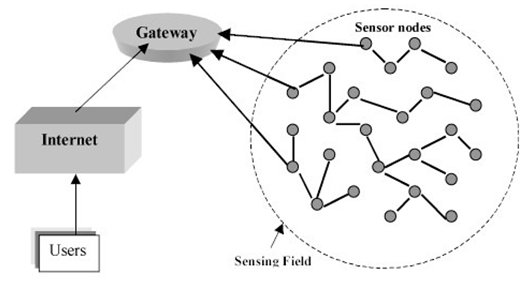
\includegraphics[scale=0.8]{Thesis/figs/wsn.png}
    \caption{Wireless sensor networks}
    \label{fig:my_label}
\end{figure}
\par
Sensor nodes are low power devices equipped with one or more sensors, a processor, memory, a power supply, a radio, and an actuator. [22] Sensors have a capability to perform limited amount of efficiency. They sense different physical conditions and send this organized data to some location. Processor performs two tasks: to process the gathered data and control the other functions of the components of a sensor nodes. Memory is used to to store the data, both application and user data. The power supply for sensor node are usually the battery cells with solar cells as their secondary backup. 
The WSNs can be classified into two categories : 
\begin{itemize}
    \item Unstructured WSNs.
    \item Structured WSNs.
\end{itemize}
Unstructured WSNs have the sensor nodes deployed in an adhoc manner i.e. randomly located in the targeted region. Strcutured WSNs, on the other hand, have the pre-planned optimal placement of sensor nodes such as grid placement.
\par \subsection{Sensor nodes hardware architecture}
This section describes the hardware architecture of the sensor nodes. Sensor nodes comprises five hardware unit viz. microcontroller unit, transmitter unit, receiver unit, sensor unit and battery unit as shown in Figure 1.2.
\begin{itemize}
    \item \textbf{Microcontroller Unit} : It is an electronic circuit which is able to perform the task and control the whole processing done within sensor node. Functionality of other components can also be controlled by microcontroller unit.
    \item \textbf{Transmitter / Receiver Unit} : The combination of transmitter and receiver unit is called transceiver unit. The transceiver unit performs in four states transmit, receive, idle and sleep state. Sensor nodes are mostly used in Industrial, Scientific and Medical (ISM) band which is globally available and provide free allocation of radio spectrum.
    \item \textbf{Sensor Unit} : Sensor perform the task of sensing the physical environment in terms of pressure and temperature. The sensing information receive from sensor are in analog form which is converted to digital signal by using analog to digital converter. Then, the converted data is sent to micorcontroller for further processing.
    \item \textbf{Battery Unit} : Sensor nodes are usually deployed in unattainable and human inaccessible environment so that the main power source of sensor nodes is battery. Energy consumed in sensor nodes for processing, sensing and communicating data to the other sensor nodes.
\end{itemize}
\begin{figure}[h!]
    \centering
    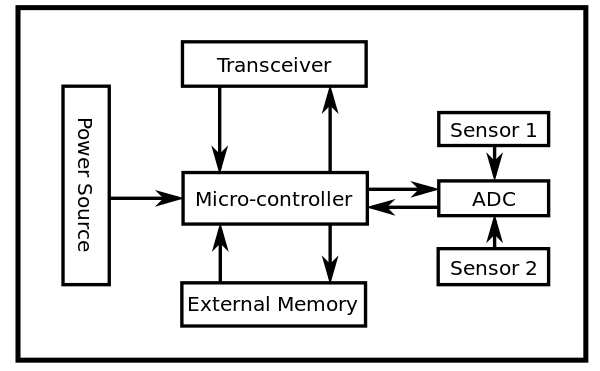
\includegraphics[scale=0.6]{Thesis/figs/10.png}
    \caption{Block diagram of sensor node hardware architecture}
    \label{fig:my_label}
\end{figure}
\subsection{Routing challenges and design issues}
\begin{itemize}
    \item Sensor nodes have limited energy resource to perform its  operations i.e. computations and transmitting information in a wireless environment.[3] Optimization of power consumption is needed in order to increase the longevity of network. This is achieved by facilitating low duty cycle operation and local signal processing. \item Fault tolerance is an important issue for WSN which arises due to failure of sensor nodes due to various reasons such as power depletion. It is necessary to maintain the network connectivity in such case. MAC and routing protocols should ensure that in case of node failures , the new data routing paths must be generated. 
    \item Radio coverage determines the connectivity of WSN. Multi-hop networking must exist between sensor nodes to reduce the chances of network partitioning and the node density must be kept sufficiently high. 
    \item WSN poses certain design issues due to the topology of the network. The random deployment of sensor nodes in the WSN region requires setup and administration to be entirely autonomous without any manual intervention.
    \item Another important issue in WSN is to maintain a good Quality of Service. Some applications are highly delay sensitive, which means that the observed data is useful as long as it is delivered within a certain time period after which it is sensed. However, some applications require a trade-off between the conservation of energy which is directly proportional to the network lifetime and the quality of service delivered. In such applications, energy-aware routing protocols come into play.
\end{itemize}
\subsection{Architecture of WSN}
Most common architecture of WSN[22] follows the OSI model as shown in Figure 1.3. It has a stack of five layers i.e. application layer, transport layer, network layer, data link layer and physical layer. Apart from these layers, there are three cross-layer for effective management of WSN i.e. task-management phase, mobility management phase and power management phase. 
\begin{figure}[h!]
    \centering
    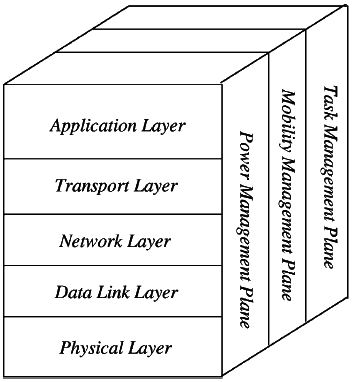
\includegraphics[scale=0.8]{Thesis/figs/architect.png}
    \caption{Architecture of Wireless sensor networks}
    \label{fig:my_label}
\end{figure}
The function of power management phase is to optimize the power consumption by turning off the various functionality of the sensor nodes in order to preserve the network energy. The task of mobility management plane is to maintain the data route to the sink in case of mobile nodes. The task management phase manages the nodes and schedules the sensing tasks of the nodes. It manages the active and idle nodes so that idle nodes can utilize their energy in routing and data aggregation. These cross layers play a very important role in  maintaining the coordination among the nodes, minimizing energy consumption and mobility of the sensor nodes.
\begin{itemize}
    \item \textbf{Physical layer} provides the carrier for data signals to be transmitted from one end to the other. Its primary responsibilities include generating carrier frequencies, signal detection and modulation and data encryption. 
    \item \textbf{Data link layer} is responsible for error detection and correction mechanisms. Furthermore, it is responsible for the channel access and buffer management policies, ensuring point-to-point or multipoint reliability. 
    \item \textbf{Network layer} is primarily responsible for routing in the network. The function of routing protocols is to find the reliable route and redundant paths in the network to minimize the cost of data transfer from source to the sink. There are various routing protocols available such as flat routing protocols and hierarchical routing protocols or time driven, event driven and query driven. 
    \item \textbf{Transport layer} function is to avoid congestion while maintaining the reliability of the network. These functionalities are provided either at the upstream or downstream i.e. from source to sink and sink to source. As WSN has limited resources, providing a hop-by-hop transmission is more efficient than end-to-end transmissions. That is why TCP are not suitable for WSN. The transport layer is particularly needed when the system is needed to gain access to other networks.
    \item \textbf{Application layer} is responsible for traffic management and provide software for different applications that translate the data in an understandable form or send queries to obtain certain information.  
\end{itemize}
\section{Motivation}
WSNs are resource constrained, therefore resource utilization has to be efficient. For fine monitoring of the sensor field parameters, nodes are densely deployed. This dense deployment results in spatial correlated traffic generation which causes congestion in the network and energy wastage.[16] In the dense WSN deployment, the density of sensor nodes is high over a given area. this allows random deployment in a critical region. In such a scenario, cooperation among the nodes is necessary. The distance between any two nodes are short and close to each other due to the dense deployment of a large number of nodes. therefore, this sensor networks exploits multi-hop communication. The problem in a dense network is that, nodes in the dense network schedule its process to prolong the network lifetime and ensure energy conservation. In the scheduling process, a reduction of active nodes results in the loss of connectivity.
\par
The focus is on applications that involve continuous data gathering for large scale and distributed physical phenomena using a dense wireless sensor network where joint routing can be more effective. An example of this is the collection of data from a field of weather sensors. If the nodes are densely deployed, the readings from nearby nodes are likely to be highly correlated as shown in Figure 1.4 and hence contain redundancies because of the inherent smoothness or continuity properties of the physical phenomenon.
Generalizing, the percentage of correlation in the data from different sources can be calculated as a function of the distance between them. \\
\begin{figure}[H]
    \centering
    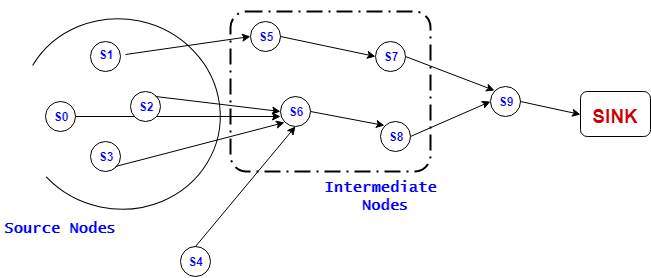
\includegraphics[scale=0.5]{Thesis/figs/moti.png}
    \caption{Sensor deployment scenario}
    \label{fig:my_label}
\end{figure}
\par
In this chapter, we have introduced WSN and its architecture. In brief we have given an overview of the whole thesis work in the introduction part and what has motivated us to take the work. The next chapter will be discussing various work in the literature for congestion control and active queue management. Following this, the research gap followed with problem formulation and objectives for our work has been specified.



\section{Thesis outline}
The outline of the research can be described as:\\
\textbf{Chapter 1} Introduction section briefly discusses the work done in the report. Then an overview of Wireless Sensor Network and its architecture have been discussed.
\\
\textbf{Chapter 2} discusses the various work done in the literature regarding congestion control and active queue management schemes. On the basis of above literature survey, research gap has been mentioned. Problem statement and our objective for the work has been given in this section.
\\
\textbf{Chapter 3} This section describes the proposed methodology to achieve our targeted objective. Mathematical validation  of the proposed approach is given in this section. Following this, we have presented the flowchart of the proposed scheme and the proposed algorithm, and they have been discussed. 
\\
\textbf{Chapter 4} This section is for the performance evaluation of our proposed work. It briefly gives an introduction to Network Simulator, the tool used for simulation. Further, the proposed mechanism has been evaluated and compared to a baseline system on various metrics and results have been discussed and analyzed.
\\
\textbf{Chapter 5} This section concludes the work done and also discusses the future work that can be carried out. 


